%!TEX root = ../MasterThesis.tex

\section{A data model for \gls{E-commerce} transactions}
\label{sec:data_model_transactions}

Based on the explanations in Chapter~\ref{cha:context_analysis}, and especially the scope definition for this Master thesis in Section~\ref{sec:scope_thesis}, the collaborative system for investigating \gls{E-commerce} fraud incidents have to answer the central question:\@

\begin{quotation}
  \textit{Is this transaction really a valid \gls{E-commerce} transaction?}
\end{quotation}

The relevant stakeholders, that need to be involved in the investigation process, are:\@

\begin{enumerate}
    \item \textbf{merchants}, who can provide additional information of each \gls{E-commerce} transaction in question
    \item \textbf{\gls{PSP}s/issuers}, that have information about the credit card usage patterns and the original credit card owners
    \item \textbf{\gls{LSP}s}, who can offer information about whether an order has already been shipped or not, and in the former case to whom it has been handed over
\end{enumerate}

Ideally each of those participants would make parts of their internal data structures available for the others to access and query for information. That would allow the stakeholder, who has to authorize or validate a suspicious credit card payment, to analyze all available information, as depicted in the Figure~\ref{fig:images_system_overview}.\@

\begin{figure}[H]
	\centering
		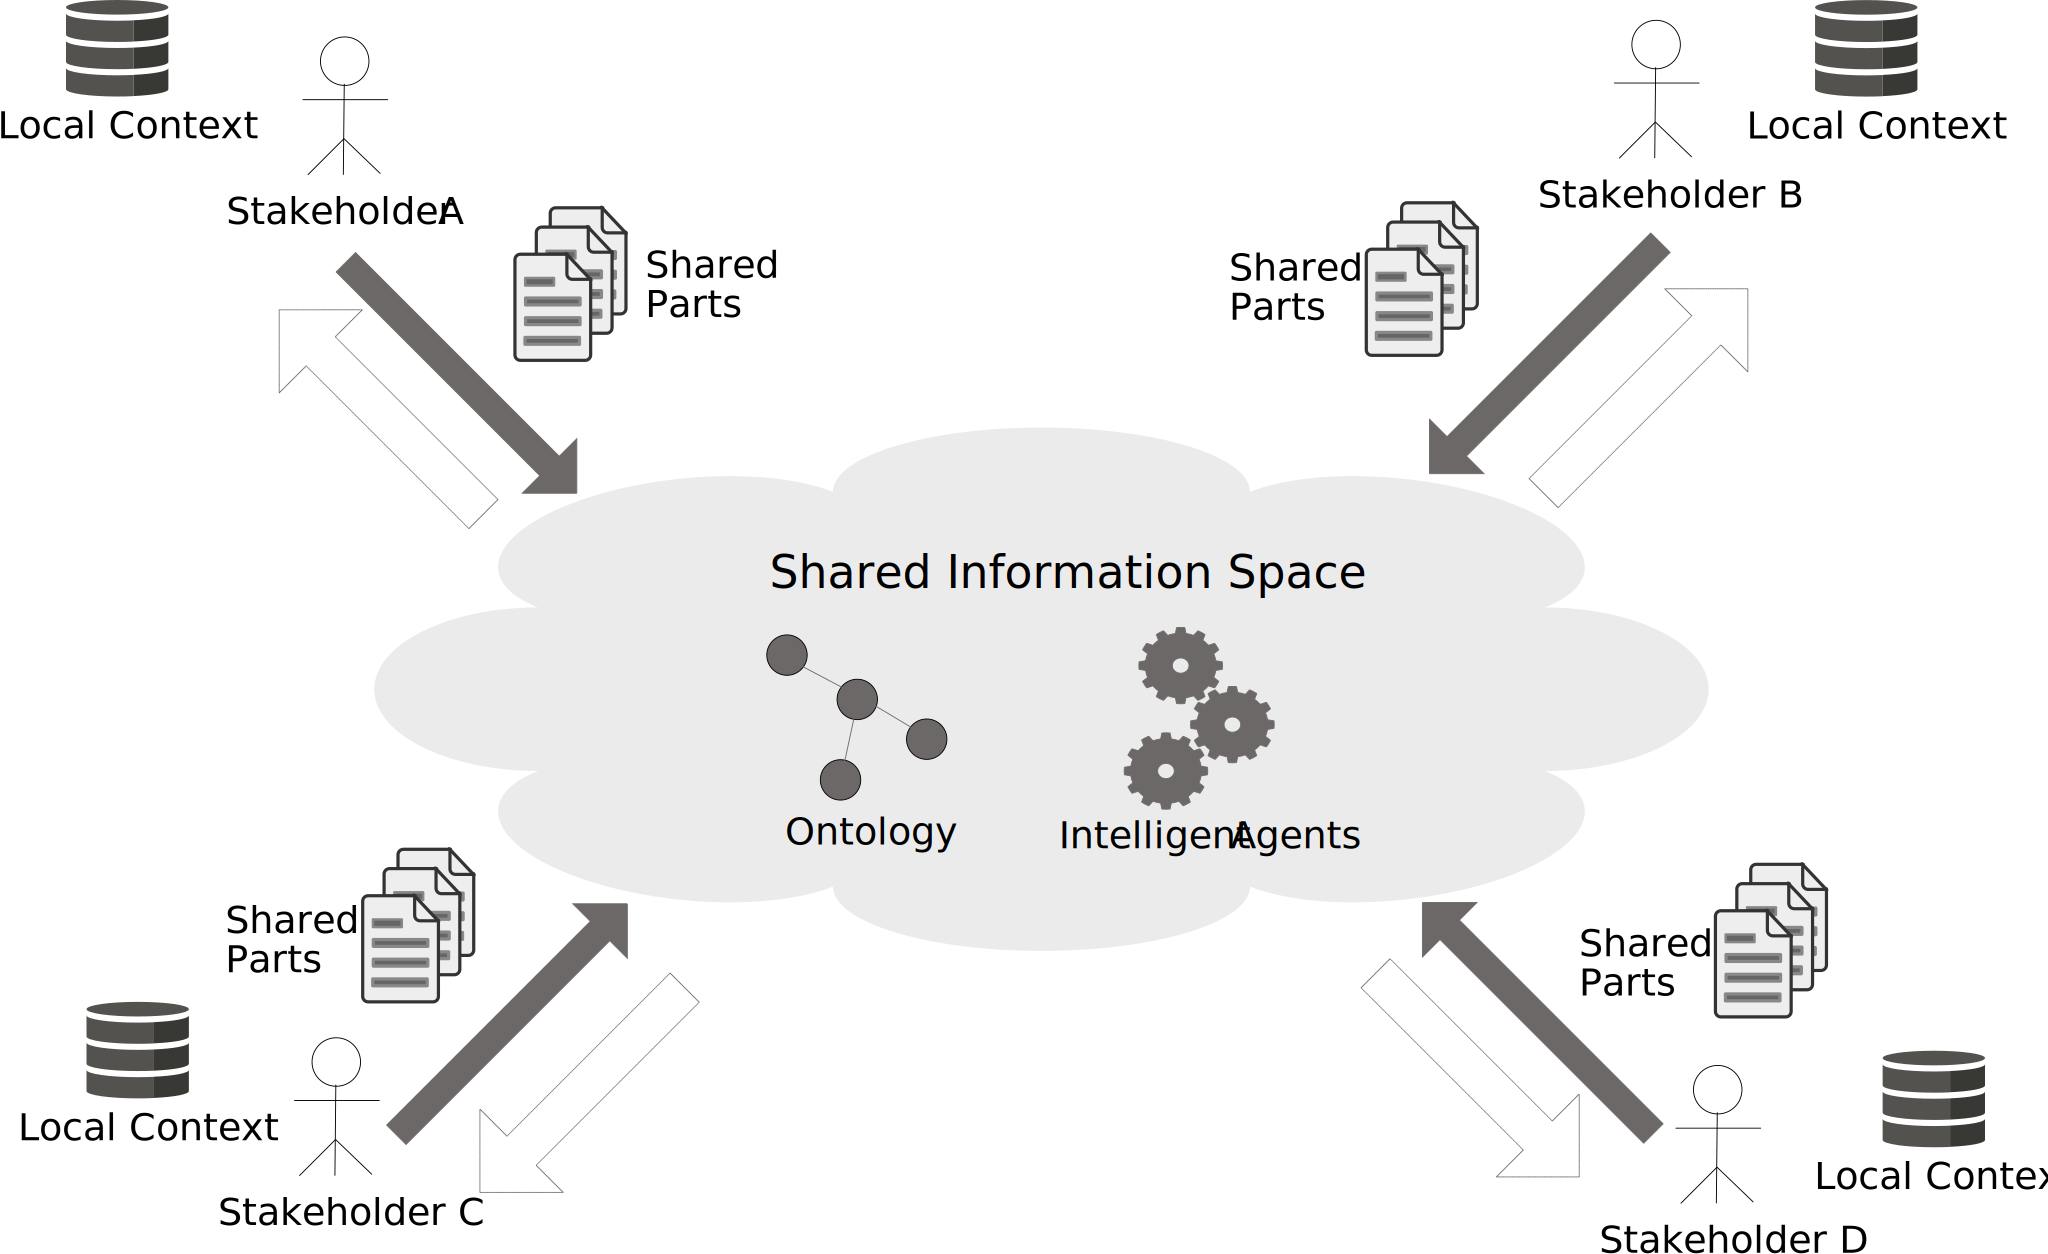
\includegraphics[width=0.9\columnwidth]{images/system_overview.pdf}
	\caption{High-level concept of the system}
\label{fig:images_system_overview}
\end{figure}

In this figure one can see that the relevant parties are providing access to parts of their internal local context information within a shared information space. Due to the fact that data from various sources have to be combined into a shared understanding of the \gls{E-commerce} activities of a consumer, there is a need to harmonize and transform the information from each participant into a shared data model to be able to analyze the combined data set. Based on this shared data model a set of intelligent agents (aka analysis algorithms) can be executed and present their findings, that can be valuable to any of the participants. \\

Based on the discussions in Chapter~\ref{cha:context_analysis}, and the analysis of the information each stakeholder holds and transmits to others, the following initial data relationships can be conducted for the \gls{E-commerce} scenario (see Figure~\ref{fig:images_data_model}). This figure shows not only the relevant information from the local contexts of each stakeholder, but also how they can be combined within a shared information space. \\

\begin{figure}[!ht]
  \centering
  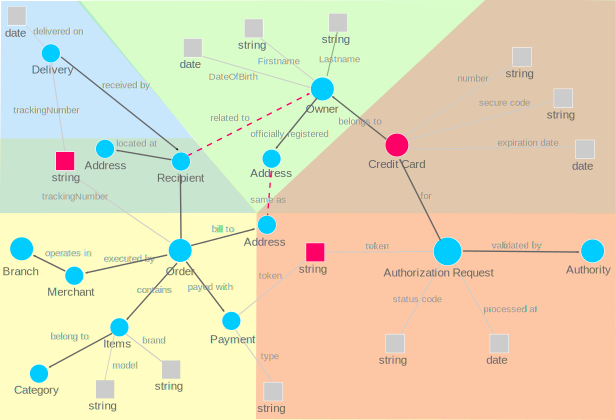
\includegraphics[width=0.9\columnwidth]{images/ontology_scenario_1.pdf}
  \caption[Data relations in the E-commerce scenario]{Data relations in the \gls{E-commerce} scenario\protect\footnotemark}
\label{fig:images_data_model}
\end{figure}

As the figure also shows there are shared information tokens between various stakeholders. Those can be used in the collaborative system as a reference for joining the distributed pieces of information into a combined view of the \gls{E-commerce} transactions. There are actually three important tokens: \@

\begin{enumerate}
  \item \textbf{payment token}: shared between merchants and \gls{PSP}s
  \item \textbf{tracking number}: shared between merchants and \gls{LSP}s
  \item \textbf{credit card}: shared between issuers and \gls{PSP}s
\end{enumerate}

In addition to these tokens the Figure~\ref{fig:images_data_model} also shows the important validation criteria. These are connections that have an influence on the decision whether an \gls{E-commerce} transaction is evaluated as suspicious or not. The two main criteria are: \@

\begin{enumerate}
  \item \textbf{billing address-to-owner address}: the billing address of the order has to match the registered address of the owner of the credit card used
  \item \textbf{recipient-to-owner}: the recipient of the delivery has to be related to the owner of the credit card
\end{enumerate}

Whereas the first criteria can be examined during the payment authorization process of an \gls{E-commerce} transaction based on the information transmitted between merchants and \gls{PSP}s or issuers, the second one is more difficult to validate (or can not be verified at all). The only check the \gls{LSP}s are able to do, before they are handing over the packaged items to the recipients, is to verify that they are the ones mentioned in the shipping address information of the order. If a recipient is somehow related to the owner of the credit card used for paying an order, or just a deceiver misusing a credit card can not be confirmed by the \gls{LSP}. \\

Also merchants, \gls{PSP}s and issuers have no possibility to check for this criteria. Whereas the merchants are able to validate whether a consumer has send items to a shipping address before, they can not restrict consumers to choose only validated recipient addresses for their orders. Doing so will have a negative impact on the business success of the online merchants. The \gls{PSP}s and issuers can not analyze this situation either, as both participants will not receive any information about the delivery address of an order with the payment authorization request from a merchant.

% section system_overview (end)
